\documentclass[../main.tex]{subfiles}
\graphicspath{{\subfix{images/}}}

\begin{document}
	\section{Sorting networks preliminaries}
	A comparator network with n inputs is a sequence of comparators, each comparator is formed by a tuple of channels $C=(i_1,j_1);...;(i_k,j_k)$ where $(1 \leq i_l < j_l \leq n)$. We name size, $S(n)$, to the number of comparators the network has. An input $\bar{x}=x_1...x_n \in \{0, 1\}^n$ outputs the network as follows: $\bar{x_0}=\bar{x}$ for $0<l\leq k$, $\bar{x^l}$ is a permutation of $\bar x^{l-1}$ exchanging $\bar x^{l-1}_{i_l}$ and $\bar x^{l-1}_{j_l}$ if $\bar x^{l-1}_{i_l} > \bar x^{l-1}_{j_l}$
	A comparator network is a sorting network if for any n inputs the outputs are the ascending ordered sequence. The reason we take only binary sequences is because of the zero-one principle\cite{knuth1997art} which states that a comparator network orders all sequences in \{0,1\} if and only if it sorts all sequences in any ordered set such as the integers set. This also allows to test if a comparator network is a sorting network without testing n! combination of sequences. If a comparator network tests all the binary sequences in 1-n it is enough to state that it is indeed a sorting network.
	
	\begin{figure}[H]
		\centering
		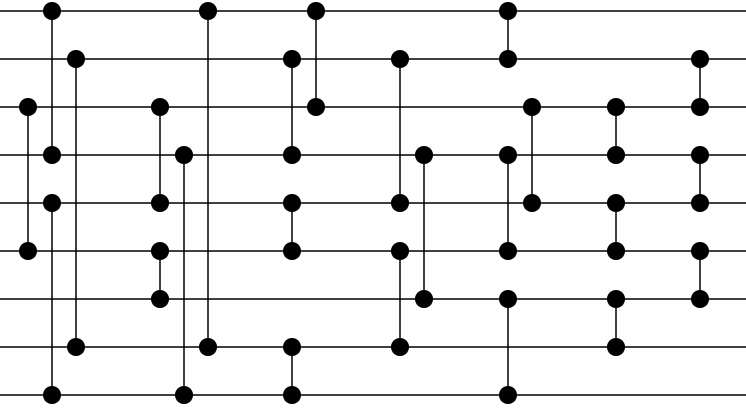
\includegraphics[scale=0.8]{images/Size8SortingNetwork}
		\caption{Size 8 sorting network}
		\label{fig:images/Size8SortingNetwork}
	\end{figure}

	As stated before the creation of sorting networks with optimal size is the problem of finding networks with the smallest possible set of comparators. Until this date optimal size sorting networks exist for $n \leq 12$, in \cite{FLOYD1973163} Floyd and Knuth found optimal size sorting networks for $n \leq 8$. In \cite{sortingnineinputs} the optimal size networks for $n = 9$ and $n = 10$ are proved and \cite{harder2021answer} proves the optimal size networks for $n = 11$ and $n = 12$ using SAT encoders. The following lemma \cite{VanVoorhis1972} is used to establish lower size bounds:
	
	\begin{lemma}
		$Size(n+1) \geq Size(n) + \log_2 n$ for all $n \geq 1$
	\end{lemma}

	Using the above lemma the sizes of S(10) was implied from S(9) in \cite{sortingnineinputs} and the size of S(12) was implied from S(11) in \cite{harder2021answer}.
	
	The method followed in this thesis is same than the one used in \cite{sortingnineinputs}. It makes use of the symmetries present in comparator networks to reduce the search space. These symmetries are formed by the permutation of channels. Given a comparator network $C=c_1;c_2;..;c_k$ with size $n$ where $c=(i_t;j_t)$ with $i\leq j \leq n$ and a permutation $\pi$. $\pi(C)$ is the sequence $\pi(c_1);...;\pi(c_k)$. We call $\pi(C)$ a generalized comparator network. This networks have the same properties than comparator networks with the exception that $i_t$ can be bigger than $j_t$. In \cite{knuth1997art} an algorithm to convert any generalized sorting network to a standard sorting network with same size and depth is proposed. 
	
	To prove the size of $S(n)$ we need to create a finite set of comparator networks that contains a sorting network. In the naive approach this set is all the comparator networks with n channels. In the next section I will explain how to reduce this set exploiting the symmetries in comparator networks. 
	
	
	
\end{document}